\documentclass[conference]{IEEEtran}
\usepackage{amsmath,amssymb}
\usepackage{graphicx}
\usepackage{booktabs}
\usepackage{siunitx}
\usepackage{cite}
\usepackage[hidelinks]{hyperref}
\graphicspath{{../results/}}
\sisetup{group-digits=false}
\setlength{\textfloatsep}{8pt plus 2pt minus 2pt}
\setlength{\abovedisplayskip}{4pt}\setlength{\belowdisplayskip}{4pt}

\begin{document}
\title{Splitting an EMT Simulation at a Line:\\Interface Delay and Thevenin Equivalents}
\author{\IEEEauthorblockN{Haoran Liu}
\IEEEauthorblockA{CloudDRTS preparation, Phase 3}}
\maketitle

\begin{abstract}
A small EMT test circuit is split at its lossless line into two solvers that exchange only the Bergeron history terms. Without added delay the split solution equals the unsplit one to round-off, and communication latency up to the line travel time minus one step costs no accuracy. Additional delay acts as extra line length: the simulation remains stable, but the error grows roughly with frequency times delay. A resistive Thevenin equivalent of one side is wrong already in steady state, a fundamental-frequency equivalent during transients, and model and delay errors do not add. A plan for the Kundur two-area system is outlined.
\end{abstract}
\begin{IEEEkeywords}
Co-simulation, distributed real-time simulation, electromagnetic transients, interface delay, network equivalents.
\end{IEEEkeywords}

\section{Introduction}
Distributing a real-time simulation over several computers or sites requires cutting the network into parts that exchange boundary quantities over a communication link~\cite{syed,stevic}. How accurately this works depends on where the network is cut, what is exchanged, how late it arrives, and how the rest of the system is represented on each side~\cite{ren2011,ren2008}. This note studies these questions on the smallest meaningful example: a circuit with one lossless line, cut at the line, with an artificial delay added at the interface and, in a second variant, one side replaced by a Thevenin equivalent.

\section{Test Circuit and Partition}
\begin{figure*}[!t]
\centering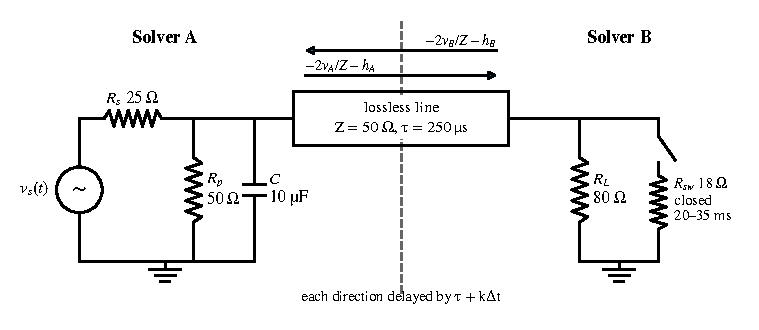
\includegraphics[width=0.62\textwidth]{phase3_circuit.pdf}
\caption{Test circuit and partition. Each solver sends one value per step to the other.}
\label{fig:circuit}
\end{figure*}
The circuit of Fig.~\ref{fig:circuit} is solved with the nodal solver of Phase~2. Side A contains a source $v_s(t)=\SI{100}{V}\,\sin(2\pi f t)$ with $f=\SI{60}{Hz}$ unless stated otherwise, $R_s=\SI{25}{\ohm}$ and a shunt $R_p=\SI{50}{\ohm}$ in parallel with $C=\SI{10}{\micro\farad}$; side B contains a load $R_L=\SI{80}{\ohm}$ and a shunt $R_{sw}=\SI{18}{\ohm}$ that closes at \SI{20}{ms} and opens at \SI{35}{ms}. The line has $Z=\SI{50}{\ohm}$ and $\tau=\SI{250}{\micro\second}$, and the time step is $\Delta t=\SI{5}{\micro\second}$, so $\tau=N\Delta t$ with $N=50$. Table~\ref{tab:contract} defines the interface.

\begin{table}[!b]
\caption{Interface Between the Two Solvers}
\label{tab:contract}
\centering\footnotesize\setlength{\tabcolsep}{3pt}
\begin{tabular}{@{}p{0.27\columnwidth}p{0.66\columnwidth}@{}}
\toprule
Item & Definition\\
\midrule
Exchanged value & outgoing history $-2v/Z-h$ of each line end, one value per direction and step\\
Sign convention & currents positive into the line, $i=v/Z+h$\\
Timing & value produced at step $n$ is used at step $n+N+k$\\
Order in a step & read incoming history, solve, send outgoing history\\
Start & steady state of the configuration (Sec.~\ref{sec:init})\\
\bottomrule
\end{tabular}
\end{table}

\section{Method}
\subsection{Interface delay}
With $k$ added steps, the history used at end $A$ is
\begin{equation}
h_A(n)=-\frac{2\,v_B(n-N-k)}{Z}-h_B(n-N-k),
\end{equation}
and likewise at end $B$. This is exactly the Bergeron model of a line with travel time $\tau+k\Delta t$, so the delayed simulation represents a longer, still lossless and passive line.

\subsection{Thevenin equivalents of side A}
Seen from the line end, side A has the impedance and open-circuit voltage
\begin{equation}
Z_\mathrm{th}(j\omega)=\frac{1}{1/R_s+1/R_p+j\omega C},\qquad E_\mathrm{th}=\frac{Z_\mathrm{th}}{R_s}\,V_s .
\end{equation}
Two equivalents are compared with the full model:
\begin{itemize}
\item \emph{Resistive}: $C$ is ignored, $e(t)=\frac{R_p}{R_s+R_p}v_s(t)$ behind $R_s\parallel R_p=\SI{16.7}{\ohm}$.
\item \emph{Phasor}: $Z_\mathrm{th}$ and $E_\mathrm{th}$ are evaluated at the source frequency. At \SI{60}{Hz}, $Z_\mathrm{th}=16.60-j1.04~\Omega$ is realized as \SI{16.60}{\ohm} in series with \SI{2543}{\micro\farad}, and $e(t)=0.665\,v_s(t)$ shifted by $-3.6^\circ$.
\end{itemize}

\subsection{Initialization and error measures}\label{sec:init}
Every run starts from the sinusoidal steady state of its own configuration with the switch open. It is computed from phasors of the discretized circuit: capacitors use the warped frequency $\omega_d=\frac{2}{\Delta t}\tan\frac{\omega\Delta t}{2}$ of the trapezoidal rule, and the line, including the added delay, the exact two-port admittances
\begin{equation}
Y_{s}=\frac{-j\cot\varphi}{Z},\quad Y_{m}=\frac{j}{Z\sin\varphi},\quad \varphi=\omega(N+k)\Delta t .
\end{equation}
The waveforms before \SI{20}{ms} are then exact sinusoids; their fitted phasors match the prediction within \SI{7e-11}{V}. Errors are evaluated for the receiving-end voltage $v_B$ against the unsplit solution. The steady-state error is $|\Delta V_B|/|V_B|$ from the phasors fitted before the event; the transient error is the relative RMS error from \SI{20}{ms} to the end of the run at \SI{50}{ms}.

\section{Results}
\begin{figure*}[!t]
\centering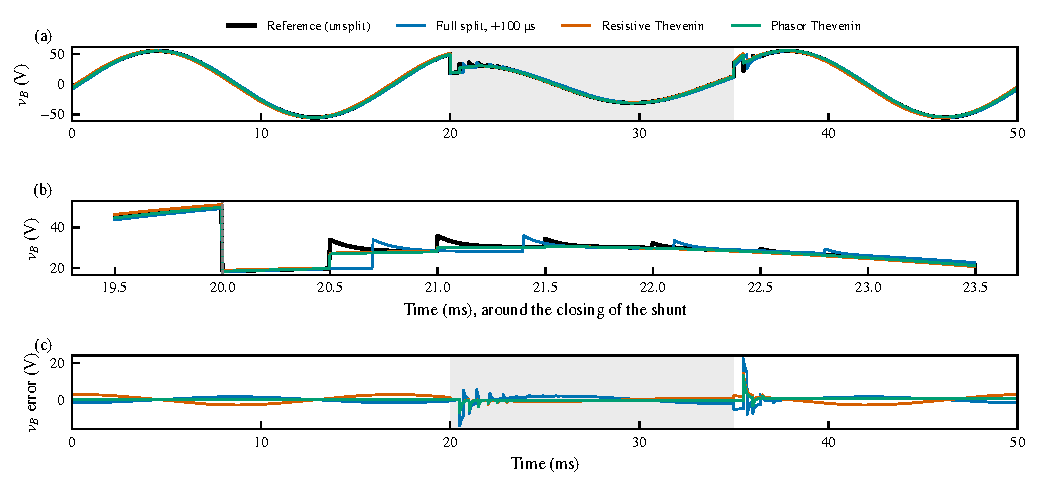
\includegraphics[width=\textwidth]{phase3_waveforms.pdf}
\caption{Receiving-end voltage at \SI{60}{Hz}: (a) complete run, shunt closed in the shaded interval; (b) first reflections after the shunt closes; (c) difference from the unsplit solution.}
\label{fig:wave}
\end{figure*}
\subsection{Split without added delay}
The split and unsplit solutions agree within \SI{2e-14}{V}. Because $\tau\ge\Delta t$, the line already decouples the nodal equations of the two sides, so cutting there involves no approximation. In real time the travel time is also a latency budget: the value needed at step $n$ is produced at step $n-N$, so communication latency up to $\tau-\Delta t\approx\SI{245}{\micro\second}$, one step being reserved for computation, has no effect on accuracy.

\subsection{Added delay}
By (1), extra delay lengthens the line. The coupled simulation stays passive and stable for any $k$, unlike voltage--current interfaces~\cite{ren2008}, but the result changes (Figs.~\ref{fig:wave} and~\ref{fig:delay}). In steady state the error grows almost linearly with the delay: \SI{0.15}{\percent} per step, \SI{3.0}{\percent} at \SI{100}{\micro\second} and \SI{12}{\percent} at \SI{400}{\micro\second} at \SI{60}{Hz}. It scales with $\omega k\Delta t$ (Fig.~\ref{fig:freq}): at \SI{100}{\micro\second} it reaches \SI{24}{\percent} at \SI{400}{Hz} and \SI{77}{\percent} at \SI{1200}{Hz}, close to the value $2\sin(\omega k\Delta t/2)$ of a pure time shift (3.8, 25 and \SI{74}{\percent}). The admissible delay depends on the highest frequency the study must reproduce.

After the switching event, the reflections between the two line ends arrive $2k\Delta t$ later in every round trip (Fig.~\ref{fig:wave}b). One step of delay already gives a transient error of \SI{1.9}{\percent}, against \SI{0.15}{\percent} in steady state, and \SI{100}{\micro\second} gives \SI{7.2}{\percent}. The pointwise maximum error is of limited use for such waveforms; with one step of delay it already amounts to \SI{27}{V}, the height of a wavefront arriving one sample late.

\begin{figure}[!t]
\centering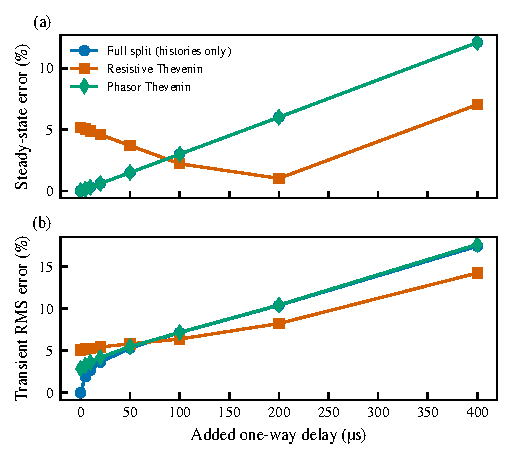
\includegraphics[width=\columnwidth]{phase3_error_vs_delay.pdf}
\caption{Error of $v_B$ at \SI{60}{Hz} against the added delay: (a) steady state, (b) transient. In (a) the full split and the phasor equivalent coincide.}
\label{fig:delay}
\end{figure}
\begin{table}[!t]
\caption{Error of $v_B$ at \SI{60}{Hz} (\%) for 0 / 100 / \SI{400}{\micro\second} of Added Delay}
\label{tab:err}
\centering\footnotesize\setlength{\tabcolsep}{4pt}
\begin{tabular}{@{}lcc@{}}
\toprule
Variant & Steady state & Transient\\
\midrule
Full split & 0 / 3.0 / 12.1 & 0 / 7.2 / 17.4\\
Resistive equivalent & 5.2 / 2.2 / 7.0 & 5.1 / 6.4 / 14.2\\
Phasor equivalent & 0.0 / 3.0 / 12.1 & 2.9 / 7.2 / 17.6\\
\bottomrule
\end{tabular}
\end{table}

\subsection{Thevenin equivalents}
Table~\ref{tab:err} compares the variants. The resistive equivalent has a steady-state error of \SI{5.2}{\percent} without any delay (\SI{33}{\percent} at \SI{400}{Hz}, \SI{85}{\percent} at \SI{1200}{Hz}). With delay this error first decreases, to \SI{1.0}{\percent} at \SI{200}{\micro\second}, because the phase lag of the delay partly cancels the phase error of the equivalent (Figs.~\ref{fig:delay}a and~\ref{fig:freq}). This cancellation depends on frequency and does not reflect a property of the interface.

The phasor equivalent is exact in steady state at the source frequency ($10^{-6}$\,\% from the discretization), so with delay its steady-state error equals that of the full split. It fails during transients, with \SI{2.9}{\percent} error without delay (\SI{4.4}{\percent} at \SI{400}{Hz}). Because of $C$, side A acts as a short circuit for steep wavefronts, whereas the equivalent presents \SI{16.6}{\ohm}; so the reflections at side A are not reproduced (Fig.~\ref{fig:wave}b). After each event its series capacitor also retains a DC offset that decays with $(R_\mathrm{th}+R_L)C_\mathrm{th}\approx\SI{0.25}{s}$, visible in Fig.~\ref{fig:wave}c after \SI{35}{ms}.

\begin{figure}[!t]
\centering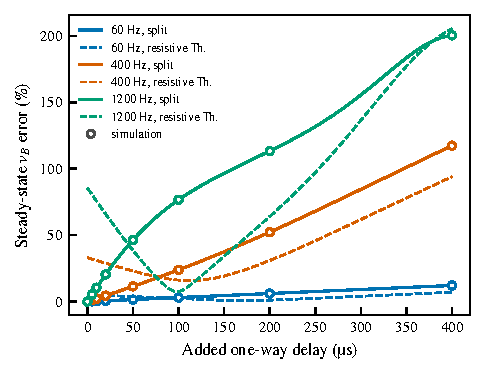
\includegraphics[width=\columnwidth]{phase3_frequency.pdf}
\caption{Steady-state error of $v_B$ against the added delay at three source frequencies. Lines: phasor solution of the continuous circuit; circles: simulation.}
\label{fig:freq}
\end{figure}

\subsection{Model error and delay error}
The two error sources do not add. For the resistive equivalent at \SI{100}{\micro\second}, the transient error caused by the equivalent alone is \SI{5.1}{\percent} and that caused by the delay alone, measured against the same equivalent without delay, is \SI{5.5}{\percent}, yet the total is \SI{6.4}{\percent}. For this reason the total error, the error due to delay alone and the error due to the equivalent alone are recorded separately for every case.

\section{Proposal for the Kundur Two-Area System}
\begin{itemize}
\item \emph{Model}: EMT model of the 11-bus system of Phase~1, first balanced single-phase and then three-phase, with the six-state machines interfaced through their stator equations and the two \SI{110}{km} tie sections as Bergeron lines ($\tau\approx\SI{386}{\micro\second}$, about 8 steps at \SI{50}{\micro\second}); unsplit solution as reference.
\item \emph{Cut}: at bus 8, the middle of the tie, so that only line histories cross the interface; added delay from 0 to about \SI{1}{ms}.
\item \emph{Equivalents of area 2}: full model; \SI{60}{Hz} Thevenin equivalent at bus 8; frequency-dependent network equivalent fitted by vector fitting~\cite{vf}, with the machines first at constant EMF and then aggregated into one machine.
\item \emph{Disturbance and metrics}: the bus-8 fault of Phase~1. EMT metrics: RMS error of the bus voltages and tie currents during the fault and the first cycles after clearing. Electromechanical metrics: frequency and damping of the inter-area mode estimated from the tie power, and the first rotor-angle swing, compared with Phase~1.
\item \emph{Outcome}: for each metric and equivalent, the largest delay that keeps the error below an agreed limit, e.g., 0.1 percentage points of inter-area damping.
\end{itemize}

\section{Conclusion}
Cutting at a line is exact while the latency stays below the travel time minus one step. Further delay acts as additional line length; the simulation remains stable, but its accuracy decreases with frequency. A phasor equivalent is exact only in steady state and a resistive equivalent not even in steady state, so equivalents for transient studies need to represent the frequency dependence of the replaced network.

\begin{thebibliography}{1}
\bibitem{syed} M.~H. Syed \emph{et al.}, ``Real-time coupling of geographically distributed research infrastructures: Taxonomy, overview, and real-world smart grid applications,'' \emph{IEEE Trans. Smart Grid}, vol.~12, no.~2, pp.~1747--1760, 2021.
\bibitem{stevic} M.~Stevic \emph{et al.}, ``Multi-site European framework for real-time co-simulation of power systems,'' \emph{IET Gener. Transm. Distrib.}, vol.~11, no.~17, pp.~4126--4135, 2017.
\bibitem{ren2011} W.~Ren \emph{et al.}, ``Interfacing issues in real-time digital simulators,'' \emph{IEEE Trans. Power Del.}, vol.~26, no.~2, pp.~1221--1230, 2011.
\bibitem{ren2008} W.~Ren, M.~Steurer, and T.~L. Baldwin, ``Improve the stability and the accuracy of power hardware-in-the-loop simulation by selecting appropriate interface algorithms,'' \emph{IEEE Trans. Ind. Appl.}, vol.~44, no.~4, pp.~1286--1294, 2008.
\bibitem{vf} B.~Gustavsen and A.~Semlyen, ``Rational approximation of frequency domain responses by vector fitting,'' \emph{IEEE Trans. Power Del.}, vol.~14, no.~3, pp.~1052--1061, Jul. 1999.
\end{thebibliography}
\end{document}
